\section{Metric Spaces and Topology}
\index{space!metric}

\begin{definition}[induced distance]
If $d\colon X\times X \to \RR$ is a distance on $X$
and $A \subset X$,
then by restricting $d$ to $A \times A$, one still obtains (obviously) a
distance.
This restriction is called the \emph{induced distance}
\mymargin{induced distance}%
\index{distance!induced}%
from $X$ on $A$.
Thus, if $A$ is a subset of a metric space $(X,d)$, $A$ also has a metric space
structure.
\end{definition}

\begin{example}[sphere]
If $X\subset \RR^n$, the Euclidean distance of $\RR^n$ induces
on $X$ a metric space structure. If $X$ is not a vector subspace of $\RR^n$, we
thus have examples of metric spaces that are not normed spaces. For example,
the \emph{$n$-dimensional sphere}%
\mymargin{$n$-dimensional sphere}%
\index{sphere}
\[
  \mathbb S^n = \ENCLOSE{\vec x \in \RR^{n+1}\colon \abs{\vec x} = 1}
\]
is a metric space with the distance induced from $\RR^n$.

For $n=1$, it is observed that $\mathbb S^1$ is the unit circle in the plane,
for $n=2$, one obtains the usual unit sphere embedded in three-dimensional
space.
\end{example}

\begin{definition}[ball]%
\label{def:palla}%
\mymark{*}%
Let $(X,d)$ be a metric space.
For every $r>0$ and for every $x_0\in X$,
we define the \emph{ball}%
\mymargin{ball}%
\index{ball} of radius $r$ centered at
$x_0$ as the set
\[
  B_r(x_0) = \ENCLOSE{x\in X \colon d(x,x_0) < r}.
\]
\end{definition}

\begin{figure}
  \centering
  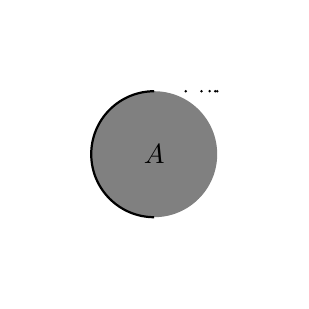
\begin{tikzpicture}[x=0.8cm,y=0.8cm]
    \draw[white] (2,-2) -- (2,2) -- (-2,2) -- (-2,-2) -- (2,-2);
    \fill[black!50] (0,0) circle (1);
    \draw[thick] (0,1) arc (90:270:1);
    \foreach \x in {0.5,0.75,0.88,0.97,1.0}
      \fill (\x,1) circle (0.5pt);
    \draw (0,0) node {$A$};
  \end{tikzpicture}
  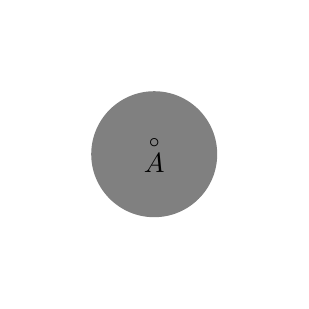
\begin{tikzpicture}[x=0.8cm,y=0.8cm]
    \draw[white] (2,-2) -- (2,2) -- (-2,2) -- (-2,-2) -- (2,-2);
    \fill[black!50] (0,0) circle (1);
    \draw (0,0) node {$\stackrel \circ A$};
  \end{tikzpicture}
  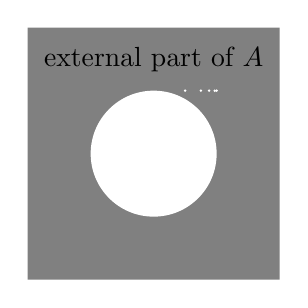
\begin{tikzpicture}[x=0.8cm,y=0.8cm]
    \fill[black!50] (2,-2) -- (2,2) -- (-2,2) -- (-2,-2) -- (2,-2);
    \foreach \x in {0.5,0.75,0.88,0.97,1.0}
      \fill[white] (\x,1) circle (0.5pt);
    \fill[white] (0,0) circle (1);
    \draw (0,1.5) node {external part of $A$};
  \end{tikzpicture}
  \begin{tikzpicture}[x=0.8cm,y=0.8cm]
    \draw[white] (2,-2) -- (2,2) -- (-2,2) -- (-2,-2) -- (2,-2);
    \foreach \x in {0.5,0.75,0.88,0.97,1.0}
      \fill (\x,1) circle (0.5pt);
    \draw[thick] (1,0) arc (0:360:1);
    \draw (0,0) node {$\partial A$};
  \end{tikzpicture}
  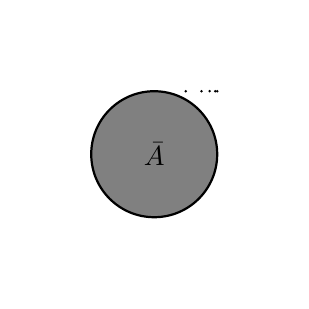
\begin{tikzpicture}[x=0.8cm,y=0.8cm]
    \draw[white] (2,-2) -- (2,2) -- (-2,2) -- (-2,-2) -- (2,-2);
    \foreach \x in {0.5,0.75,0.88,0.97,1.0}
      \fill (\x,1) circle (0.5pt);
    \fill[black!50] (0,0) circle (1);
    \draw[thick] (1,0) arc (0:360:1);
    \draw (0,0) node {$\bar A$};
  \end{tikzpicture}
  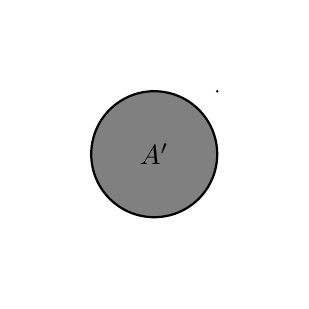
\begin{tikzpicture}[x=0.8cm,y=0.8cm]
    \draw[white] (2,-2) -- (2,2) -- (-2,2) -- (-2,-2) -- (2,-2);
    \fill (1,1) circle (0.5pt);
    \fill[black!50] (0,0) circle (1);
    \draw[thick] (1,0) arc (0:360:1);
    \draw (0,0) node {$A'$};
  \end{tikzpicture}
\caption{A set $A$
and its interior $\stackrel \circ A$,
external part, boundary $\partial A$, closure $\bar A$, and accumulation points
$A'$.}
\label{fig:}
\end{figure}

\begin{definition}[topological relations and properties]%
\mymark{*}%
\label{def:466342}%
Let $(X,d)$ be a metric space.
A set $A\subset X$ is said to be an
\emph{open}%
\mymargin{open}%
\index{open} set in $X$ if for every $x\in A$, there exists $r>0$
such that $B_r(x) \subset A$.
A set $A\subset X$ is said to be a
\emph{closed}%
\mymargin{closed}%
\index{closed} set in $X$ if its complement $X\setminus A$ is open.

The family of all open sets is called the \emph{topology}%
\mymargin{topology}%
\index{topology} of the metric space $X$. 
All the following definitions do not depend on the distance $d$ but only on the
topology:
it suffices to use arbitrary open sets instead of the balls $B_r(x)$.

If $A\subset X$ is any set
and $x\in X$ is any point, we say that:
\begin{enumerate}
\item
$x$ is an \emph{interior point}%
\mymargin{interior point}%
\index{point!interior} of $A$ if there exists $r>0$ such that $B_r(x) \subset A$;
we call the
\emph{interior}%
\mymargin{interior}%
\index{interior}
of $A$ the set of interior points of $A$
and denote it by $\stackrel\circ A$;
\item
$A$ is a \emph{neighborhood}%
\mymargin{neighborhood}%
\index{neighborhood} of $x$ if $x$ is an interior point of $A$,
i.e., there exists $r>0$ such that $B_r(x)\subset A$;
\item
$x$ is an \emph{exterior point}%
\mymargin{exterior point}%
\index{point!exterior} of $A$ if it is interior to the complement of $A$, i.e., there exists $r>0$ such that $B_r(x) \cap A = \emptyset$;
we call the \emph{exterior}%
\mymargin{exterior}%
\index{exterior} of $A$ the set of exterior points of $A$;
\item
$x$ is a \emph{boundary point}%
\mymargin{boundary point}%
\index{point!boundary} for $A$ if it is neither interior nor exterior to $A$, i.e., for every $r>0$, the set $B_r(x)$ contains points of $A$ and of $X\setminus A$;
we call the \emph{boundary}%
\mymargin{boundary}%
\index{boundary} (or edge) of $A$ the set of boundary points, which we denote by $\partial A$.
\item
$x$ is an \emph{adherent point}%
\mymargin{adherent point}%
\index{point!adherent} of $A$ if it is interior or a boundary point, i.e., for every $r>0$, we have $B_r(x) \cap A \neq \emptyset$;
we call the \emph{closure} of $A$ the set of adherent points,
which we denote by $\bar A$;
\mymargin{closure}%
\index{closure}
\index{closure}
\item
$x$ is an \emph{accumulation point}%
\mymargin{accumulation point}%
\index{point!accumulation} of $A$ if
it is an adherent point for $A \setminus \ENCLOSE{x}$, i.e.,
for every $r>0$, the set $A \cap B_r(x)$ contains points different from $x$, we
call the \emph{derived set}%
\mymargin{derived set}\index{derived set} of $A$ the set of accumulation points (which could be denoted by $A'$);
\item
$x$ is an \emph{isolated point}%
\mymargin{isolated point}\index{point!isolated} of $A$ if it is a point of $A$ but not an accumulation point for $A$, i.e., if there exists $r>0$ such that
$B_r(x) \cap A = \ENCLOSE{x}$.
\end{enumerate}
\end{definition}

\begin{theorem}[balls are open]
Let $(X,d)$ be a metric space, let $x\in X$ and $r>0$. Then the ball $B_r(x)$ is
an open set in $X$.
\end{theorem}
%
\begin{proof}
Let $y\in B_r(x)$: it is sufficient to find $\rho>0$ such that $B_\rho(y)
\subset B_r(x)$. Taking $\rho = r-d(y,x)$, it is observed that $\rho >0 $ and,
by the triangle inequality,
given $z \in B_\rho(y)$, we have
\[
  d(z,x) \le d(z,y) + d(y,x) < \rho + d(y,x) = r
\]
from which $B_\rho(y)\subset B_r(x)$ as we wanted to prove.
\end{proof}